\documentclass[11pt]{article}
\usepackage{eadca-template}
\usepackage[plain]{algorithm}

\usepackage[brazil,english]{babel}
\usepackage[utf8]{inputenc}
\usepackage[T1]{fontenc}

\usepackage{graphicx,url}
\usepackage[hang]{subfigure}
\usepackage{psfrag}
\usepackage{booktabs}
\usepackage[
    breaklinks=true,    
    allbordercolors=blue,
%    ocgcolorlinks=true,
    colorlinks=true,
    anchorcolor=blue, 
    citecolor=blue,
    filecolor=blue,
    linkcolor=blue,
    menucolor=blue,
    runcolor=blue,
    urlcolor=blue,
    linktoc=all
]{hyperref}
\makeatletter
    \g@addto@macro{\UrlBreaks}{\do\/\do\-\do\_}
\makeatother
\usepackage[ocgcolorlinks]{ocgx2}

\sloppy


\title{Resolução de CAPTCHA's utilizando Redes Neurais Convolucionais}

\author{Rafael Gonçalves \and Thomás Portugal}

\address{Departamento de Engenharia de Computa\c{c}\~{a}o e Automa\c{c}\~{a}o Industrial (DCA) \\
  Faculdade de Engenharia El\'{e}trica e de Computa\c{c}\~{a}o (FEEC) \\
  Universidade Estadual de Campinas (Unicamp)\\
  CEP 13083-852 -- Campinas, SP, Brasil
  \email{\{ra186062,ra187646\}@.fee.unicamp.br}}

\hyphenation{}
\pagestyle{fancy}

\begin{document}

%%%%%%%%%%%%%%%%%%%%%%%%%%%%%%%%%%%%%%%%%%%%%%%%%%%%%%%%%%%%%%%%%%%%%%%%%%%%%
\twocolumn[
\maketitle
\thispagestyle{fancy}
\selectlanguage{english}

   \begin{abstract}
       This project studies the possibility of using k-means and convolutional neural networks for solving text-based reverse Turing test mechanism, called CAPTCHA. Such mechanism is often used in network security for preventing attacks such as password guessing using bruteforce or dictionary or denial of service attacks.
       Our approuch was based on creating a pipeline of pre-processing, segmentation and optical character recognition. For the first part of the project we used otsu threshold, erosion and dilatation methods for denoising, then used k-means clusterization algorithm for segmentation and finally trained a convolutional neural network to classify each individual character. The output was the concatenation of the output of the network for each input character of the CAPTCHA.
   \end{abstract}

  \keywords{CAPTCHA,  k-means, otsu threashold, convolutional  neural  networks, network security, optical character recognition.}
]
%%%%%%%%%%%%%%%%%%%%%%%%%%%%%%%%%%%%%%%%%%%%%%%%%%%%%%%%%%%%%%%%%%%
\selectlanguage{brazil}

  \section{Introdu\c{c}\~{a}o}
  \label{sec:introducao}

CAPTCHA (\em Completely Automated Public Turing test to tell Computers and Humans Apart\em ) é um mecanismo utilizado em serviços digitais para garantir que softwares automatizados não peçam acesso em excesso ou de maneira torpe, preservando a integridade e a confiabilidade de tais serviços. Normalmente um CAPTCHA é uma imagem gerada por um computador, com caracteres distorcidos. A intenção é que seja uma tarefa relativamente fácil para uma pessoa executar, mas razoavelmente complicada, do ponto de vista computacional.

Como o CAPTCHA vem sendo extensamente usado como a primeira linha de defesa contra ataques DDoS (\em Distributed Denial of Services\em ) e afins, saber o quanto essa ferramenta é segura no contexto atual é de suma importância.
Este trabalho visa desenvolver um sistema, baseado em redes neurais convolucionais e em um algoritmo de clusterização, para a identificação dos caracteres apresentados em imagens de CAPTCHA coletadas do banco de dados do site Kaggle \cite{data}.

  %%%%%%%%%%%%%%%%%%%%%%%%%%%%%%%%%%%%%%%%%%%%%%%%%%%%%%%%%%%%%%%%%%
  \section{Proposta}
  \label{sec:detalhes}

  O problema principal foi dividido em dois subproblemas: um de segmentação de imagem utilizando uma algoritmo de aprendizado não supervisionado (clusterização) e outro de classificação de imagens. Estes foram baseados em \cite{kopp2017}.

Antes da segmentação da imagem, houve um trabalho de pré-processamento dos dados baseado em \cite{proc}. Foram aplicados filtros para diminuir o nível de ruído da imagem, facilitando o trabalho de segmentação. 

A parte de clusterização envolveu determinar em que regiões da imagem estavam os caracteres. Em imagens geradas por CAPTCHA, frequentemente, há sobreposição de letras e números, além de ruídos e manchas que não representam caracter nenhum. Estas artimanhas são utilizadas justamente para dificultar a ação de algoritmos sobre as imagens. Com o uso de clusterização, os caracteres foram identificados e a imagem foi cortadas para o uso posterior na etapa de classificação. 

Na etapa de classificação, os fragmentos selecionados na etapa anterior, são separados em treino e teste, e inseridos na entrada de uma rede neural. Essa rede neural foi treinada para identificar os dígitos individualmente. Após ser aplicada nas amostras de teste, os caracteres foram identificados e a previsão da imagem juntou as saídas individuais de cada amostra e identificou os caracteres gerados pelo CAPTCHA originalmente.



\subsection{Pré Processamento}
\label{sec:preprocessing}

Antes de tudo foram aplicadas técnicas de processamento de imagem para remover possíveis distorções e ruídos e facilitar a segmentação não supervisionada da imagem.

Nossa abordagem consistiu em aplicar um filtro que melhor convertesse a imagem em preto e branco a fim de remover as influências do degradê em cinza no fundo da imagem e posterior aplicação de filtros de \em erosion \em e \em dilatation \em visando remover linhas artificialmente adicionadas por cima dos caracteres (Figura ~\ref{fig:preproc}).

  \begin{figure}[H]
        {\centering
        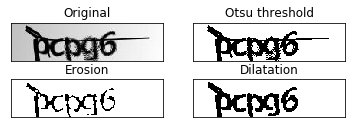
\includegraphics[width=70mm]{images/preproc.png}
        \caption{Etapas usadas para preprocessamento.}
        \label{fig:preproc}\par}
  \end{figure}

Foram testados 3 filtros diferentes (Figura ~\ref{fig:filters}) para a primeira etapa (\em adaptative threshold\em , filtro Otsu e filtro Otsu com ruído aleatório adicionado) e diferentes valores de iterações para os filtros de \em erosion \em e \em dilatation\em . Os filtros escolhidos, a saber filtro Otsu com 1 iteração de cada uma das distorções apresentadas, foram os que melhor removeram o ruído, selecionados por inspeção visual em uma amostra aleatória das imagens.

  \begin{figure}[H]
        {\centering
        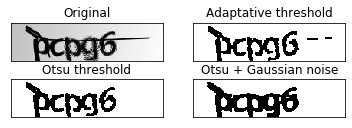
\includegraphics[width=70mm]{images/filters.png}
        \caption{Resultado do preprocessamento para cada filtro com erosion e dilatation.}
        \label{fig:filters}\par}
  \end{figure}


\subsection{Segmentação da Imagem em Caracteres}
\label{sec:cluteri}

Para separar os caracteres presentes na imagem processada, foi utilizado um algoritimo de clusterização e posteriormente expandiu-se um retângulo ao redor dos centroides dos clusters para determinar a região da imagem a ser salva como um caractere.

A abordagem escolhida para a etapa de clusterização foi o algoritmo k-means. O dataset utilizado, tinha a especificação de apenas de 5 caracteres por imagem. Assim, o número de 5 clusters foi determinado previamente. Por existir caracteres sobrepostos, a clusterização não identificava as fronteiras entre os caracteres de maneira tão eficiente. Além disso, o algoritmo, recorrentemente, identificava clusters na vertical, o que não é adequado já que os caracteres são dispostos na horizontal (Figura ~\ref{fig:kmeans2d}). 

A solução encontrada foi projetar os dados no plano horizontal e em seguida aplicar o k-means apenas em 1 dimensão. Com isso, a informação utilizada de fato foi a posição horizontal dos centroides. Para cortar as imagens os centros foram posicionados no meio do eixo vertical (Figura ~\ref{fig:kmeans1d}).

  \begin{figure}
        {\centering
        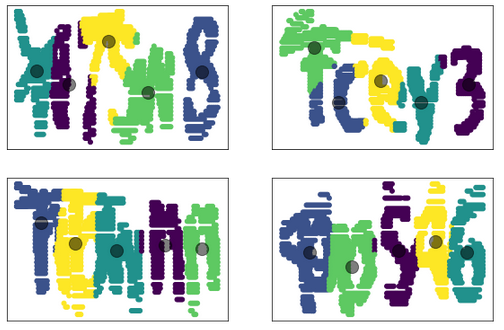
\includegraphics[width=70mm]{images/2dkmeans.png}
        \caption{Clusters encontrados pelo kmeans nas 2 dimensões das imagens.}
        \label{fig:kmeans2d}\par}
  \end{figure}

  \begin{figure}
        {\centering
        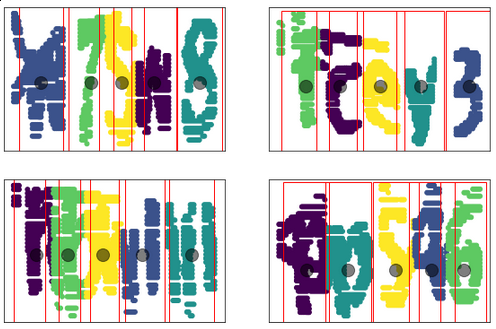
\includegraphics[width=70mm]{images/1dkmeans.png}
        \caption{Clusters encontrados pelo kmeans no eixo horizontal. Retangulo ao redor de cada caractere encontrado pelo kmeans.}
        \label{fig:kmeans1d}\par}
  \end{figure}

Com as posições do centro, foi necessário determinar os tamanhos para realizar o corte na imagem. Através de tamanhos pré-estabelecidos, foi determinado o tamanho de 21 pixels a direita e a esquerda do centro gerado pelo k-means. Essas imagens foram utilizadas na entrada da rede neural. 

\subsection{Reconhecimento de Caracteres}
\label{ssec:convnet}

A etapa de reconhecimento de caracteres consistiu em uma rede neural convolucional inspirada em \cite{kopp2017}. A rede possui a seguinte arquitetura:

\begin{enumerate}
\item
    Duas camadas convolucionais com kernel de lado 5, função de ativação linear retificada e max-polling de 2. A primeira com 6 kernels e a segunda com 16 kernels.
\item
    Duas camadas intermediárias \em fully connected \em com respectivamente 400 e 340 neurônios ReLU e dropout de 30\%
\item
    A camada de saída com 19 neurônios e função de ativação softmax
\end{enumerate}

  \begin{figure}[H]
        {\centering
        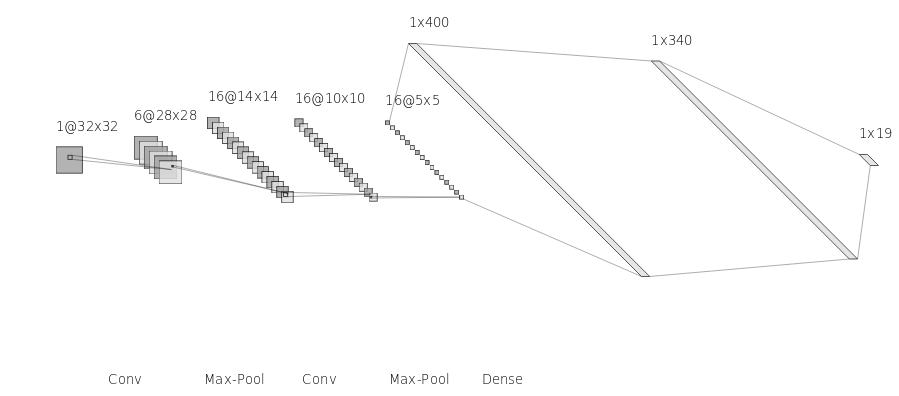
\includegraphics[width=70mm]{images/nn.png}
        \caption{Arquitetura da rede neural.}
        \label{fig:nn}\par}
  \end{figure}

O modelo foi escolhido usando validação cruzada (k-fold) e foi o que obteve a maior acurácia média entre os valores testados tanto para número de neurônios da última camada intermediária quanto para o valor de dropout (Tabela ~\ref{ex}).

\begin{table}[H]
    {\centering
\begin{tabular}{@{}lll@{}}
\toprule
H   & Dropout & Avg Accuracy \\ \midrule
50  & 0       & 0.8719       \\
50  & 0.3     & 0.9197       \\
50  & 0.5     & 0.9008       \\
120 & 0       & 0.8996       \\
120 & 0.3     & 0.9444       \\
120 & 0.5     & 0.9499       \\
340 & 0       & 0.9048       \\
340 & 0.3     & 0.9541       \\
340 & 0.5     & 0.9382       \\ \bottomrule
\end{tabular}
\caption{Comparação entre modelos testados. H é o número de neurônios na última camada intermediária da rede neural.}
\label{tab:ex}
    \par}
\end{table}

\section{Resultados}

Como mostrado na Tabela ~\ref{tab:ex}, a acurácia do modelo de reconhecimento de caracteres foi de $0.9541$ - a curva de aprendizado do modelo com o valor da função de custo pelo número de épocas está mostrado na Figura ~\ref{fig:learning} e algumas predições na Figura ~\ref{fig:pred}.

  \begin{figure}[H]
        {\centering
        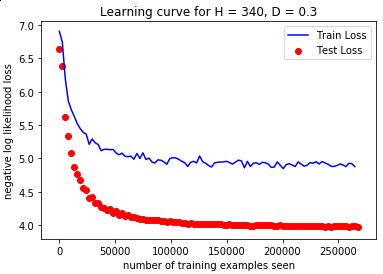
\includegraphics[width=70mm]{images/learning.png}
        \caption{Curva de aprendizado da rede neural.}
        \label{fig:learning}\par}
  \end{figure}

  \begin{figure}[H]
        {\centering
        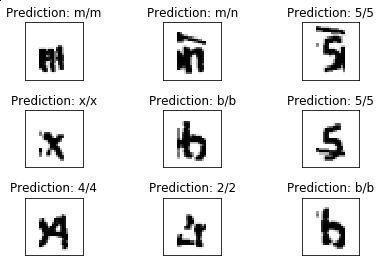
\includegraphics[width=70mm]{images/pred.png}
        \caption{Classes encontradas pela rede neural para alguns caracteres individuais de entrada.}
        \label{fig:pred}\par}
\end{figure}

A acurácia do modelo completo (classificação do CAPTCHA todo) foi de $0.3246$. Algumas das predições podem ser vistas na Tabela ~\ref{tab:pred} 


\begin{table}[H]
    {\centering
\begin{tabular}{@{}ll@{}}
\toprule
Output   & Target \\ \midrule
g7w6y &g7wxw \\
6cn48 &62nb4 \\
6byng &6bxwg \\
gpbwn &dpbyd \\
wm47f &wm47f \\
ybncw &wbncw \\
532fm &5325m \\ \bottomrule
\end{tabular}
    \caption{Comparação entre resultados previstos e rótulos para o modelo final.}
\label{tab:pred}
    \par}
\end{table}


A matriz de confusão (Figura ~\ref{fig:confusion}) aponta que a maior parte das predições incorretas tem a ver com os caracteres 'm' e 'n'. Analisando-se os resultados foi possível perceber que $37\%$ das predições incorretas ($25\%$ das predições totais) foram causadas por confusões entre esses dois caracteres.

  \begin{figure}[H]
        {\centering
        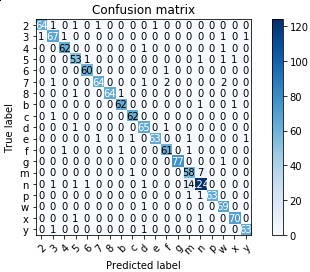
\includegraphics[width=70mm]{images/confusion.png}
        \caption{Matriz de confusão para a saída da rede neural.}
        \label{fig:confusion}\par}
  \end{figure}




\section{Conclus\~{o}es}

Foi possível desenvolver um sistema que identifica imagens de CAPTCHA com uma acurácia total de $0.3246$ para os dados contidos no \em dataset \em \cite{data}. O valor é baixo comparado com os valores atingidos por outros modelos de classificação de textos, mas mostra uma vulnerabilidade bastante relevante presente no tipo de CAPTCHA analisado. Para trabalhos posteriores, podem ser testados outros modelos de clusterização para que este englobe CAPTCHA’s com diferentes números de caracteres. Na parte de reconhecimento de caracteres, podem ser testadas redes neurais com diferentes arquiteturas, bem como outros modelos de classificação. É possível também que os métodos aqui desenvolvidos sejam usados em conjunto com bancos de dados com mais imagens para melhorar seu desempenho.
% Outra melhoria que pode ser feita é o uso de outras métricas que levem em conta um banco de dados com classes desbalanceadas.

%%%%%%%%%%%%%%%%%%%%%%%%%%%%%%%%%%%%%%%%%%%%%%%%%%%%%%%%%%%%%%%%%%%%%%%%%%%%%
\nocite{15min} 
  \bibliographystyle{plain}

   \bibliography{bib-template}

\end{document}
